\documentclass{standalone}
\usepackage{tikz}
\usepackage{ctex,siunitx}
\setCJKmainfont{Noto Serif CJK SC}
\usepackage{tkz-euclide}
\usepackage{amsmath}
\usetikzlibrary{patterns, calc}
\usetikzlibrary {decorations.pathmorphing, decorations.pathreplacing, decorations.shapes,}
\begin{document}
\small
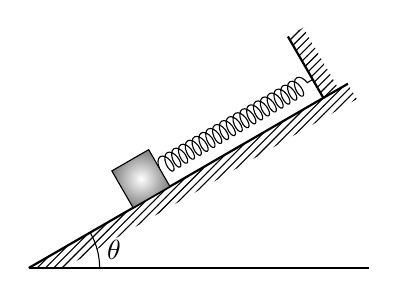
\begin{tikzpicture}[>=stealth,scale=0.9]
  % \useasboundingbox(-0.25,-0.25)rectangle(4,3);
  \tikzstyle{spring}=[decorate,decoration={aspect=0.5, segment length=1mm, amplitude=1.2mm,coil}]
  \draw[thick](0,0)--(4.8,0);
  \draw[thin](1.0,0)arc(0:30:1.0)node[midway,right]{$\theta$};
  \begin{scope}[rotate=30] 
    \fill [pattern = north east lines] (5.05,0) rectangle (4.8,1);
    \fill [pattern = north east lines] (0,0) --++(-30:0.5)-- (5.2,-0.25)--(5.2,0);
    \draw[thick](4.8,0)--(4.8,1); 
    \draw[thick](0,0)--(5.2,0); 
    \draw [spring](2.3,.3)--(4.8,.3);
    \filldraw[outer color=gray,inner color=white](1.7,0)rectangle(2.3,0.6);
  \end{scope}
\end{tikzpicture}
\end{document}